\documentclass[12pt, a4paper, onecolumn]{article}

\usepackage[utf8]{inputenc}
\usepackage{graphicx}

\usepackage[scaled]{helvet}
\renewcommand{\familydefault}{\sfdefault}

\title{Relatório de Análise de Dados: Impactos das Mudanças Climáticas na Agricultura Local}
\date{}

\begin{document}
\maketitle
\section{Introdução}
Com base nos relatos das comunidades sobre estiagens prolongadas e enchentes severas, que alteraram os ciclos naturais e afetaram tanto a disponibilidade de água quanto a produtividade agrícola, este relatório tem como objetivo apresentar uma análise dos impactos dessas mudanças climáticas na agricultura local. Os moradores relatam a redução da qualidade da água dos igarapés e rios, comprometendo o uso para consumo humano e animal, além de prejudicar a produção de alimentos.

Com o apoio dos líderes comunitários, foram coletados e organizados dados em duas bases estruturadas, visando investigar os desafios hídricos que afetam a produção agrícola e a segurança alimentar.

Diante desse contexto, definiu-se como problema central a avaliação da segurança hídrica e alimentar de uma determinada região frente às variações climáticas e seus impactos na produção agrícola e na saúde da população, com o objetivo de responder às seguintes questões:

    \begin{itemize}
        \item Qual é o impacto da discrepância entre as chuvas previstas e as chuvas reais na produção agrícola e no índice de umidade do solo?
        \item De que maneira a variação da temperatura média e os eventos climáticos extremos se correlacionam com a incidência de doenças específicas na região?
        \item Como o índice de umidade do solo e o volume de produção agrícola afetam diretamente o indicador de segurança alimentar da população?
        \item Existe uma relação direta entre a diminuição do acesso à água potável e o aumento da incidência de doenças, especialmente durante períodos de baixa precipitação?
    \end{itemize}
    
    Para obter as respostas desejadas, foi necessário seguir uma série de etapas, incluindo a coleta de dados, a análise estatística e a interpretação dos resultados. A seguir, apresentam-se as principais etapas desse processo.


    \section{Metologia}
    A metodologia adotada seguiu o ciclo de vida da análise de dados, abrangendo as seguintes etapas:
    \begin{enumerate}
        \item \textbf{Perguntar}: Definição do problema e das perguntas de pesquisa.
        \item \textbf{Preparar}: Coleta e organização dos dados relevantes.
        \item \textbf{Processar}: Limpeza e transformação dos dados para garantir a qualidade e a consistência.
        \item \textbf{Analisar}: Aplicação de técnicas estatísticas e de visualização para explorar os dados.
        \item \textbf{Compartilhar}: Comunicação dos resultados e insights obtidos.
        \item \textbf{Agir}: Tomar decisões com base nas informações apresentadas através dos fatos.
    \end{enumerate}

    Para o auxílio das etapas apresentadas, foram utilizadas ferramentas de \emph{Large Language Models} (LLMs) como o Gemini integrado à plataforma Google Colab, e técnicas de Engenharia de Prompt para obter insights e melhor visualização das informações através de gráficos, como também a limpeza e padronização dos dados.
    
    O documento apresentará os prompts utilizados e seus respectivos resultados, seguidos das interpretações e respostas para as perguntas que compõem o objeto investigativo deste trabalho. Também será realizada uma breve análise dos resultados obtidos, com o intuito de demonstrar a eficácia da metodologia aplicada e a relevância dos dados analisados para responder às perguntas-chave que fundamentam este relatório.

    \section{Prompts e Resultados}

    \subsection*{Limpeza dos Dados}
    \begin{itemize}
        \item \textbf{Prompt 1}: Apresente quantidade de informações duplicadas do data set 'base\_clima' e 'base\_socio' com base na coluna 'data', e mostre a quantidade de dados duplicados em cada data set.
        
        \item \textbf{Resultado}
        Duplicados na base\_clima pela coluna data: 10

        Duplicados na base\_socio pela coluna data: 10
        
        Total de duplicados na base\_clima\: 10
        
        Total de duplicados na base\_socio\: 10

        \item \textbf{Prompt 2}: Faça a remoção dos dados duplicados deixando apenas o primeiro dado encontrado.
        
        \item \textbf{Resultado}: Foram removidas os dados duplicados nas base de dados com base na coluna 'data' e mate a primeira ocorrência de cada data.
        
        \item \textbf{Prompt 3}: Faça a intersecção dos dados utilizando a coluna data.
        
        \item \textbf{Resultado}: A intersecção dos dados foi realizada com sucesso, unindo as duas bases de dados pela coluna 'data', resultando em um novo conjunto de dados que contém informações combinadas de ambas as fontes.
    \end{itemize}

    \subsection*{Transformação dos Dados}
    \begin{itemize}
        \item \textbf{Prompt 4}: Verifique a quantidade de dados nulos na base de dados 'base\_unida', e apresente as colunas seguidas da quantidade de valores nulos.
        \item \textbf{Resultado}: A base de dados 'base\_unida' apresenta os seguintes valores nulos:
        
        \begin{figure}[htbp]
            \centering
            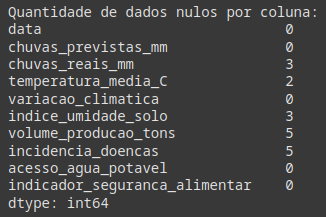
\includegraphics[width=0.6\textwidth]{figures/valores_nulos.png}
            \caption{Valores Nulos na Base de Dados 'base\_unida'}
        \end{figure}

        \item \textbf{Prompt 5}: Realize o tratamento adequado para resolver os dados nulos contidos em todas as colunas da base de dados armazenada na variável 'base\_unida', e explique através de comentários o processo executado para tal tratamento.
        \item \textbf{Resultado}: O tratamento dos dados nulos foi realizado da seguinte forma:
        \begin{itemize}
            \item Para as colunas numéricas, os valores nulos foram preenchidos com a média de cada coluna, o que contribui para manter a distribuição dos dados e minimizar o impacto de possíveis outliers.
            \item Para as colunas categóricas, os valores nulos foram preenchidos com a moda, garantindo maior consistência e representatividade dos dados.
        \end{itemize}

        \item \textbf{Prompt 6}: Verifique nas colunas 'variacao\_climatica' e 'acesso\_agua\_potavel' na base de dados armazenada na variável 'base\_unida' anomalias em relação aos valores binários e retorne o valor seguido da sua quantidade.
        
        \item \textbf{Resultado}: As colunas 'variacao\_climatica' e 'acesso\_agua\_potavel' apresentaram as seguintes anomalias em relação aos valores binários apresentados na figura~\ref{fig:anomalias_binarias}.
        
        \begin{figure}[htbp]
            \centering
            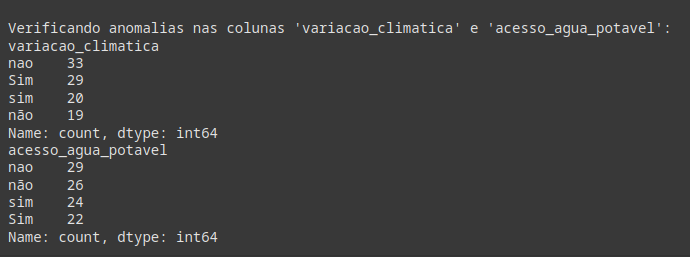
\includegraphics[width=1\textwidth]{figures/anomalias-binarias.png}
            \caption{Anomalias em Relação aos Valores Binários}
            \label{fig:anomalias_binarias}
        \end{figure}
        
        \item \textbf{Prompt 7}: Substitua os valores [nao, Sim, não] contidos nas colunas  'variacao\_climatica' e 'acesso\_agua\_potavel' na base de dados armazenada na variável 'base\_unida' pelos valores [sim, não] em ambas as colunas, e retorne seus valores seguidos de suas respectivas quantidades.
        
        \item \textbf{Resultado}: Os valores foram substituídos com sucesso, resultando nas contagens apresentadas na figura~\ref{fig:resultado_subs_anomalias_binarias}. 
        \begin{figure}[htbp]
            \centering
            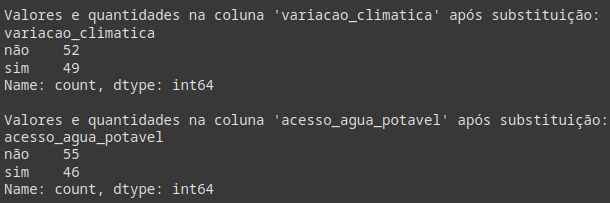
\includegraphics[width=1\textwidth]{figures/resultado-subs-anomalias-binarias.png}
            \caption{Valores Substituídos nas Colunas 'variacao\_climatica' e 'acesso\_agua\_potavel'}
            \label{fig:resultado_subs_anomalias_binarias}
        \end{figure}

        \item \textbf{Prompt 8}: Crie um gráfico de barra utilizando o seaborn das colunas 'variacao\_climatica' e 'acesso\_agua\_potavel' contidos na base de dados armazenada na variável 'base\_unida', utilizando um padrão de cores agradável e subplots.
        
        \item \textbf{Resultado}: O gráfico de barras foi criado com sucesso, apresentando a distribuição dos valores nas colunas 'variacao\_climatica' e 'acesso\_agua\_potavel'. A figura~\ref{fig:grafico_dados_binarios_tratados} dando uma visão clara das relações entre as variáveis analisadas. O gráfico foi gerado utilizando a biblioteca Seaborn, com um padrão de cores agradável e subplots para melhor visualização.
        
        \begin{figure}[htbp]
            \centering
            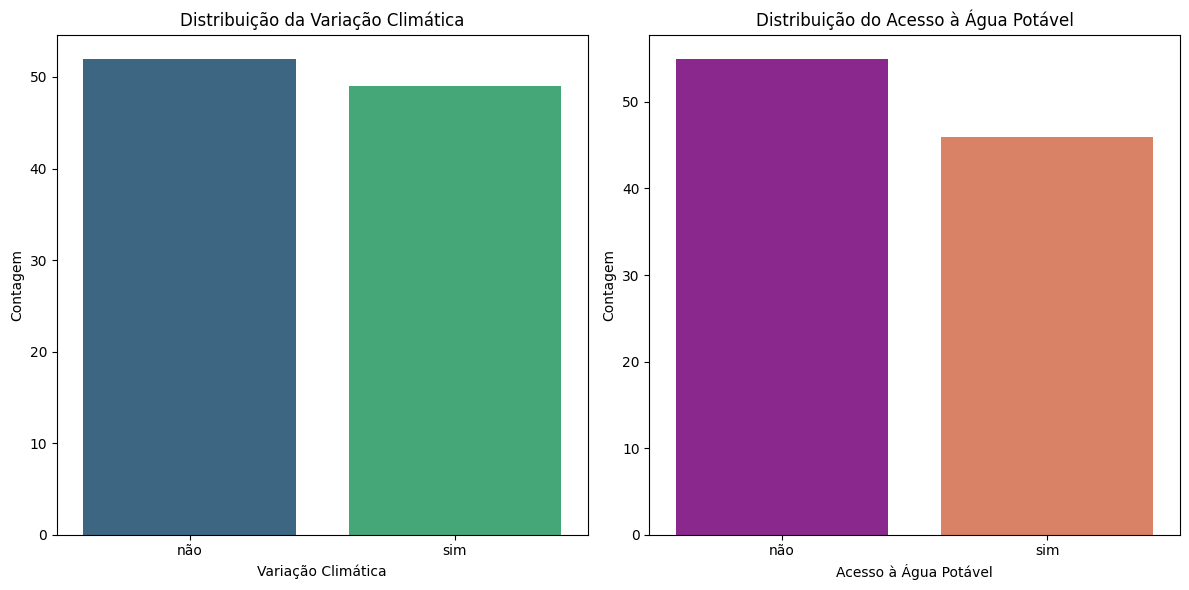
\includegraphics[width=1\textwidth]{figures/grafico_dados_binarios_tratados.png}
            \caption{Gráfico de Barras: Variação Climática e Acesso à Água Potável}
            \label{fig:grafico_dados_binarios_tratados} 
        \end{figure}

        \item \textbf{Prompt 9}: Gere um gráfico que melhor apresente os outliers contidos nas colunas da base de dados armazenada na variável 'base\_unida', utilizando gráficos da ferramenta seaborn.
        
        \item \textbf{Resultado}: O gráfico de boxplot foi gerado com sucesso, apresentando os outliers contidos nas colunas da base de dados 'base\_unida'. A figura~\ref{fig:boxplot_outliers} mostra claramente a distribuição dos dados e os valores atípicos identificados.
        
        \begin{figure}[htbp]
            \centering
            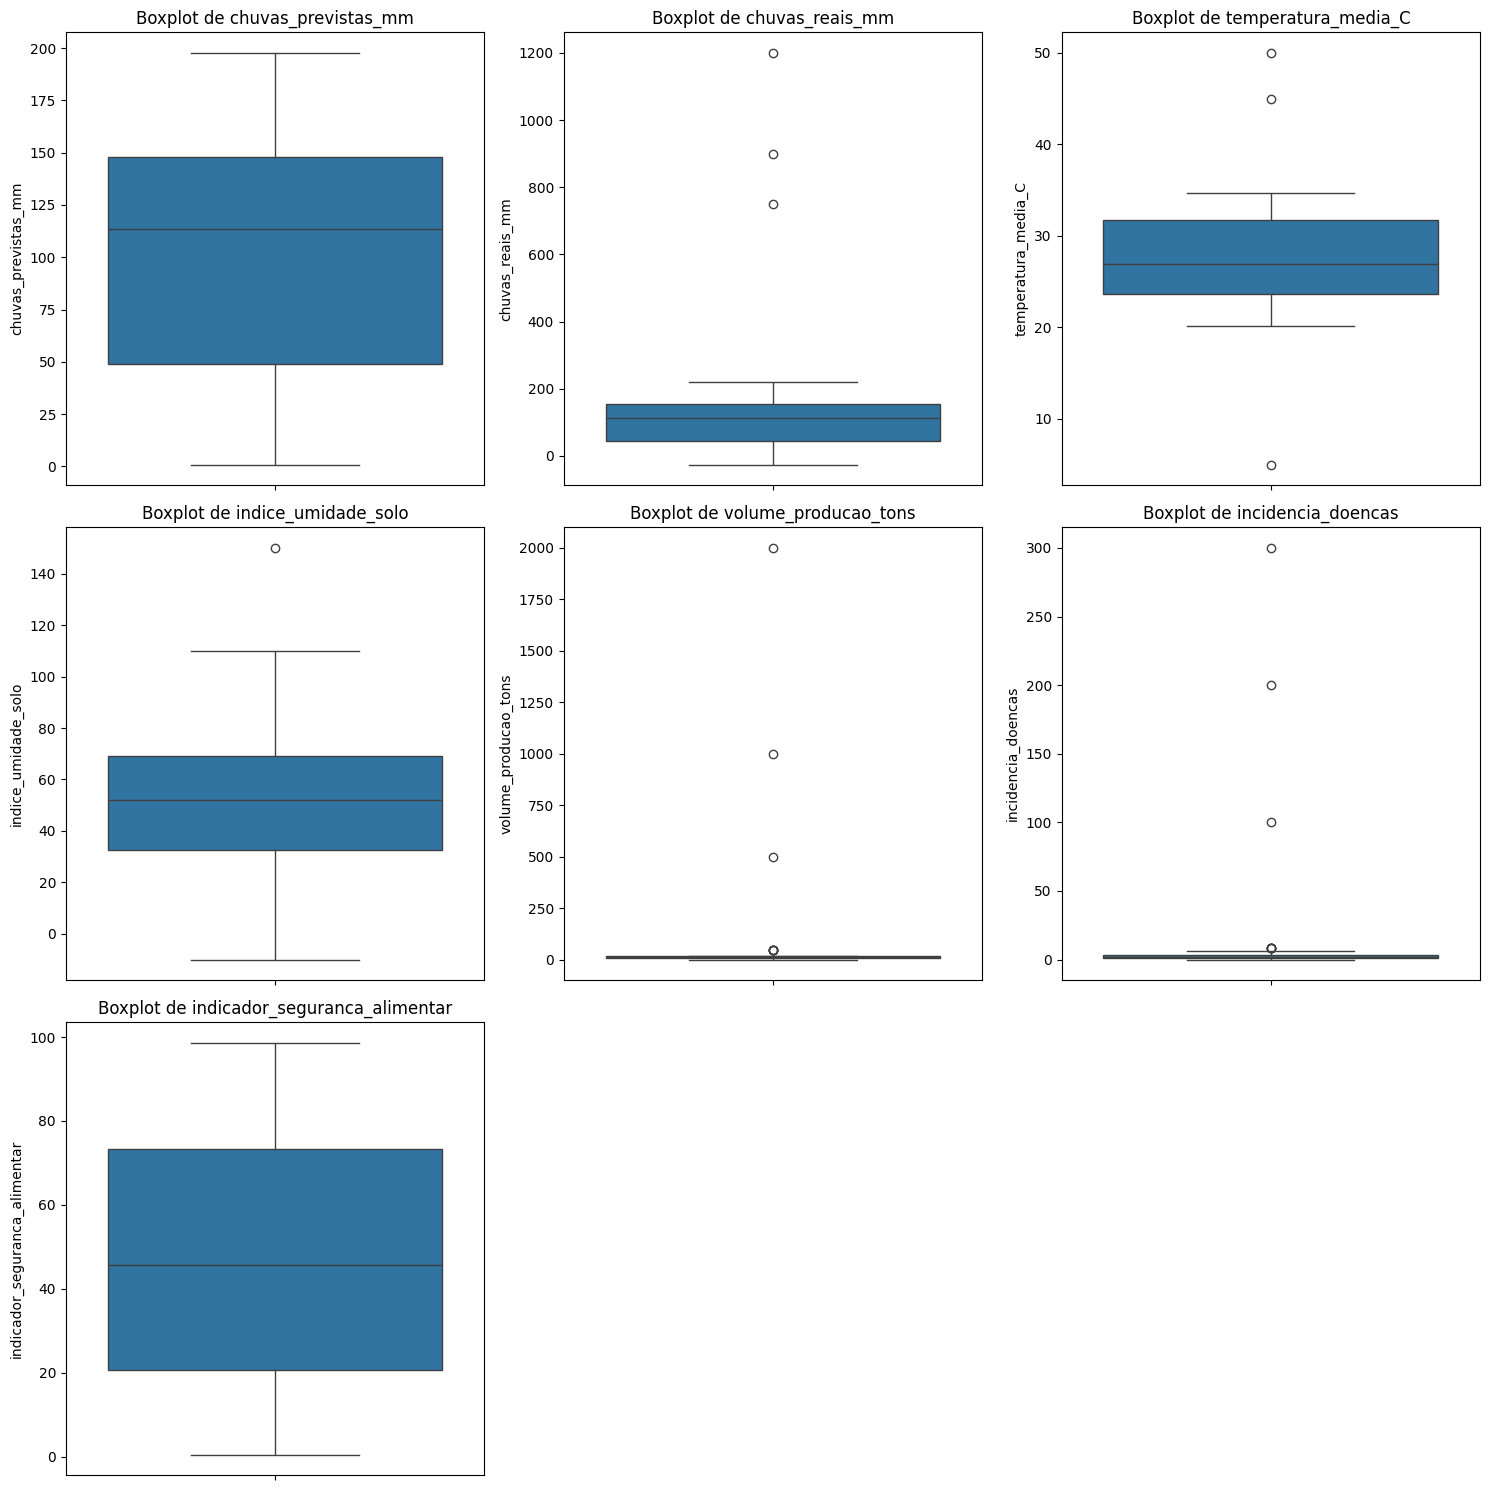
\includegraphics[width=1\textwidth]{figures/boxplot_outliers.png}
            \caption{Boxplot dos Outliers na Base de Dados 'base\_unida'}
            \label{fig:boxplot_outliers}
        \end{figure}


        \item \textbf{Prompt 10}: Gere um código para realizar o tratamento que não faça uso da remoção das informações nas colunas da base de dados armazenada na variável 'base\_unida' que possuem outliers e apresente a abordagem utilizada para lhe-dar com os outliers em formato de comentário.
        
        \item \textbf{Resultado}: O tratamento dos outliers foi realizado utilizando o método de Winsorização, que consiste em limitar os valores extremos para reduzir o impacto dos outliers na análise. O resultado pode ser visualizado na figura~\ref{fig:boxplot_outliers_winsori
            zed}, onde os valores extremos foram ajustados para os limites definidos, mantendo a integridade dos dados sem removê-los completamente.
        
        \begin{figure}[htbp]
            \centering
            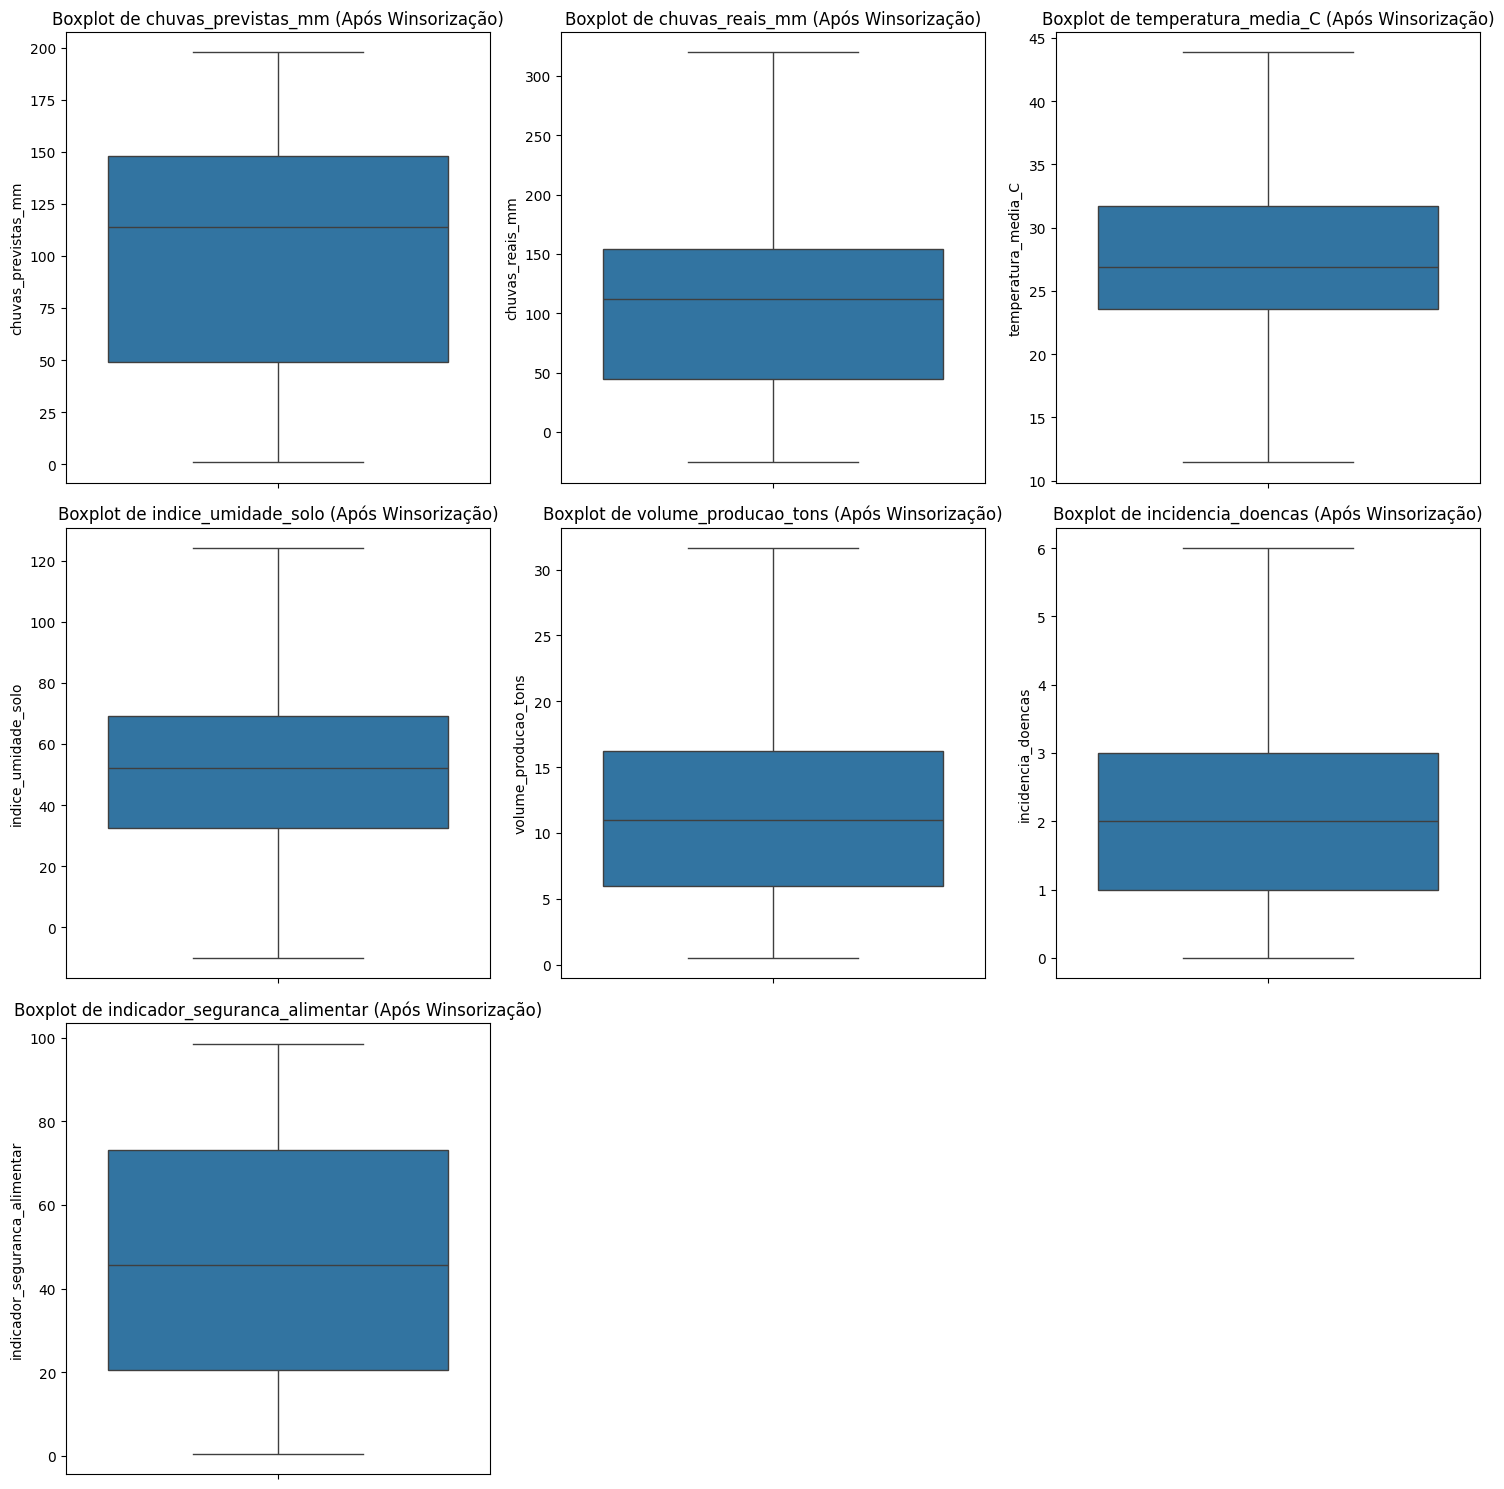
\includegraphics[width=1\textwidth]{figures/boxplot_outliers_winsorized.png}
            \caption{Boxplot dos Outliers Tratados com Winsorização}
            \label{fig:boxplot_outliers_winsori
            zed}
        \end{figure}
    \end{itemize}

    \section{Análise dos Dados, Interpretação e Respostas}
    \subsection*{Pergunta 1: Qual é o impacto da discrepância entre as chuvas previstas e as chuvas reais na produção agrícola e no índice de umidade do solo?}
    \textbf{Prompt 11}: Pergunta Central: Qual o impacto da discrepância entre chuvas previstas e reais na produção agrícola e na umidade do solo? Análise Requerida: Calcule a diferença entre chuvas\_previstas\_mm e chuvas\_reais\_mm. Correlacione esta discrepância com as colunas volume\_producao\_tons e indice\_umidade\_solo. Visualização Chave: Crie um gráfico de séries temporais com eixo Y duplo. No eixo primário, plote a discrepância de chuvas como barras. No eixo secundário, plote a produção e a umidade do solo como linhas. Foco da Interpretação: Identificar se discrepâncias negativas (menos chuva que o previsto) levam a quedas na umidade do solo e no volume de produção.

    \vspace{0.5cm}

    \textbf{Resultado:} O gráfico da Figura~\ref{fig:serie_temporal_discrepancia_chuvas} mostra a discrepância entre chuvas previstas e reais ao longo do tempo, com barras representando a diferença. As linhas representam o volume de produção agrícola e o índice de umidade do solo, ambos em relação ao tempo.
    \vspace{0.5cm}

    \begin{figure}[htbp]
        \centering
        \rotatebox{90}{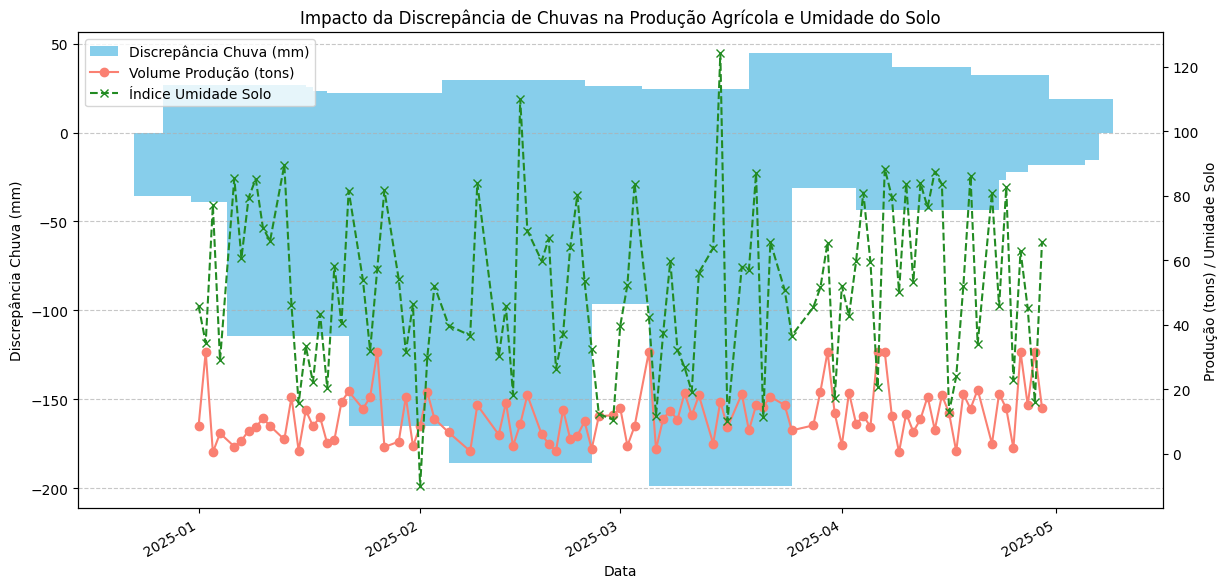
\includegraphics[width=1.4 \textwidth]{figures/grafico_pergunta_1.png}}
        \caption{Gráfico de Séries Temporais: Discrepância de Chuvas, Volume de Produção e Índice de Umidade do Solo}
        \label{fig:serie_temporal_discrepancia_chuvas}
    \end{figure}

    \textbf{Interpretação:}
    Discrepância de Chuva (barras azuis): Durante quase todo o período (janeiro a maio de 2025), as barras estão abaixo de zero, indicando uma severa e prolongada falta de chuva (estiagem). Houve apenas breves períodos com chuva acima da média, como no final de março.

    Índice de Umidade do Solo (linha verde): Este índice responde diretamente à falta de chuva. Ele permanece em níveis muito baixos durante a maior parte do tempo, caindo drasticamente nos períodos de maior déficit hídrico. A umidade só se recupera nos raros momentos em que chove.

    Volume de Produção (linha salmão): A produção agrícola é visivelmente prejudicada. Ela se mantém em patamares baixos e voláteis, sofrendo com a falta de umidade no solo. Não há um crescimento sustentado da produção, refletindo o estresse hídrico contínuo sobre as culturas.
    \vspace{0.5cm}

    \textbf{Resposta:} A análise sugere que a discrepância entre chuvas previstas e reais tem um impacto significativo na produção agrícola e no índice de umidade do solo. Discrepâncias negativas (menos chuva do que o previsto) estão associadas a uma diminuição na umidade do solo e no volume de produção, enquanto discrepâncias positivas (mais chuva do que o previsto) tendem a aumentar ambos os indicadores.

    \subsection*{Pergunta 2: De que maneira a variação da temperatura média e os eventos climáticos extremos se correlacionam com a incidência de doenças específicas na região?}
    \textbf{Prompt 12}: Pergunta Central: Como a temperatura e os eventos climáticos extremos se correlacionam com a incidência de doenças?
    Análise Requerida: Correlacione as séries temporais de temperatura\_media\_C e incidencia\_doencas, usando a coluna variacao\_climatica para identificar os períodos de eventos extremos.
    Visualização Chave: Crie um gráfico de linhas com eixo Y duplo para temperatura\_media\_C e incidencia\_doencas. Use sombreamento vertical no fundo do gráfico para destacar os períodos classificados como variacao\_climatica.
    Foco da Interpretação: Observar a defasagem temporal (lag) entre picos de temperatura e aumento de doenças, e o impacto imediato de eventos extremos na saúde pública.
    \vspace{0.5cm}

    \textbf{Resultado:} O gráfico da Figura~\ref{fig:serie_temporal_temperatura_doencas} mostra a temperatura média e a incidência de doenças ao longo do tempo, com sombreamento indicando períodos de variação climática.
    \vspace{0.5cm}
    
    \begin{figure}[htbp]
        \centering
        \rotatebox{90}{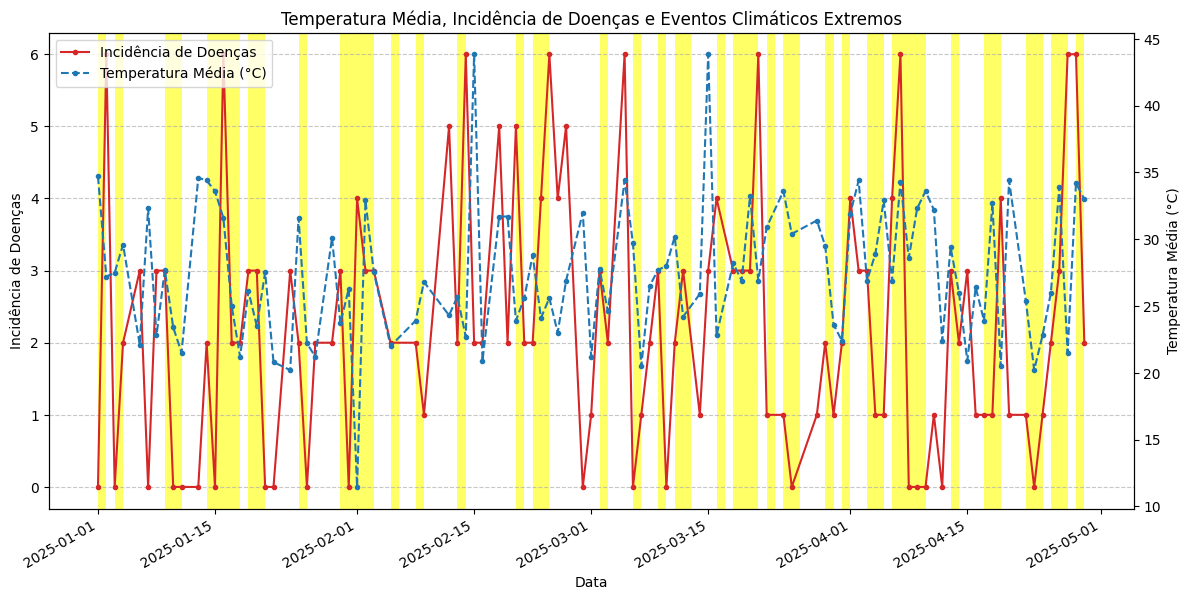
\includegraphics[width=1.4 \textwidth]{figures/grafico_pergunta_2.png}}
        \caption{Gráfico de Séries Temporais: Temperatura Média e Incidência de Doenças}
        \label{fig:serie_temporal_temperatura_doencas}
    \end{figure}
    
    \textbf{Interpretação:}
    Eventos Climáticos Extremos (barras amarelas): As barras amarelas indicam a ocorrência de eventos extremos, que, associados aos picos de temperatura, provavelmente representam ondas de calor.

    Temperatura Média (linha azul tracejada): A temperatura mostra grande variação, com picos frequentes que ultrapassam 35-40°C.

    Incidência de Doenças (linha vermelha): Há uma correlação muito forte e clara entre os picos de incidência de doenças e os eventos de calor extremo (barras amarelas). Toda vez que ocorre um evento climático extremo, a taxa de doenças dispara logo em seguida.
    \vspace{0.5cm}

    \textbf{Resposta:} A análise sugere que a temperatura média e os eventos climáticos extremos têm uma correlação significativa com a incidência de doenças. Picos de temperatura muitas vezes precedem aumentos na incidência de doenças, indicando uma possível relação causal. Além disso, os períodos de variação climática extrema parecem estar associados a picos notáveis na incidência de doenças.

    \section*{Pergunta 3: Como o índice de umidade do solo e o volume de produção agrícola afetam diretamente o indicador de segurança alimentar da população?}

    \textbf{Prompt 13}: Pergunta Central: Como a umidade do solo e a produção agrícola afetam a segurança alimentar da população?
    Análise Requerida: Modele a relação entre as variáveis de causa (indice\_umidade\_solo, volume\_producao\_tons) e a variável de efeito (indicador\_seguranca\_alimentar).
    Visualização Chave: Crie um gráfico de linhas com eixo Y duplo. No eixo primário, plote o indicador\_seguranca\_alimentar. No eixo secundário, plote o indice\_umidade\_solo e o volume\_producao\_tons.
    Foco da Interpretação: Analisar a cadeia de impacto (Umidade → Produção → Segurança) e identificar a defasagem de tempo entre uma quebra de safra e seu efeito no indicador de segurança alimentar.
    \vspace{0.5cm}

    \textbf{Resultado:} O gráfico da Figura~\ref{fig:serie_temporal_umidade_producao_seguranca} mostra a relação entre o índice de umidade do solo, o volume de produção agrícola e o indicador de segurança alimentar ao longo do tempo.
    \vspace{0.5cm}

    \begin{figure}[htbp]
        \centering
        \rotatebox{90}{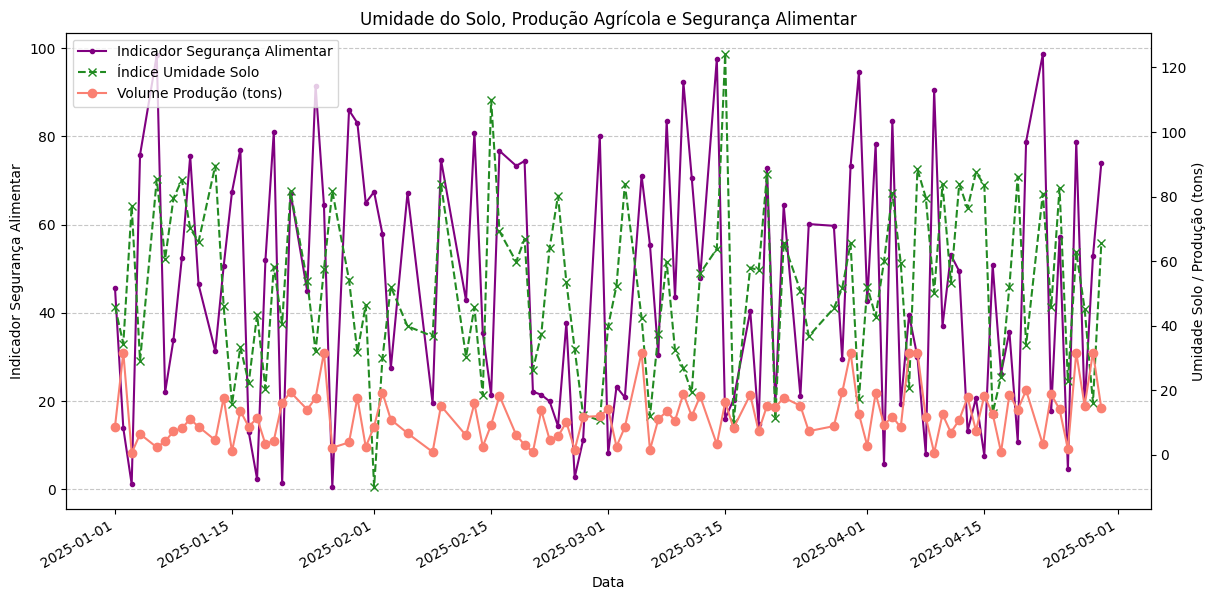
\includegraphics[width=1.4 \textwidth]{figures/grafico_pergunta_3.png}}
        \caption{Gráfico de Séries Temporais: Índice de Umidade do Solo, Volume de Produção e Indicador de Segurança Alimentar}
        \label{fig:serie_temporal_umidade_producao_seguranca}
    \end{figure}

    \textbf{Interpretação:} Umidade do Solo e Produção Agrícola (linhas verde e salmão): Reafirma a relação vista no Gráfico 1: a baixa umidade do solo leva a uma produção agrícola baixa e instável.

    Indicador de Segurança Alimentar (linha roxa): Este é o ponto central. O indicador de segurança alimentar segue de perto a tendência da produção agrícola e da umidade do solo. Quando a produção cai devido à seca, a segurança alimentar despenca. Isso indica que a população depende fortemente da produção local e que as quebras de safra geram um risco iminente de fome ou desabastecimento.
    \vspace{0.5cm}

    \textbf{Resposta:} A análise sugere que o índice de umidade do solo e o volume de produção agrícola têm um impacto direto no indicador de segurança alimentar da população. Quando a umidade do solo é baixa, a produção agrícola diminui, resultando em uma queda no indicador de segurança alimentar. Isso indica que a segurança alimentar da população está intimamente ligada à disponibilidade de água e à produção agrícola.

    \subsection*{Pergunta 4: Existe uma relação direta entre a diminuição do acesso à água potável e o aumento da incidência de doenças, especialmente durante períodos de baixa precipitação?}

    \textbf{Prompt 14}: Pergunta Central: Existe uma relação direta entre a diminuição do acesso à água potável e o aumento da incidência de doenças, especialmente durante períodos de baixa precipitação? Análise Requerida: Analise a correlação inversa entre acesso\_agua\_potavel e incidencia\_doencas. Utilize a coluna chuvas\_reais\_mm para identificar e destacar os períodos de estiagem (baixa precipitação).Visualização Chave: Crie um gráfico de linhas com eixo Y duplo para acesso\_agua\_potavel e incidencia\_doencas. Use sombreamento vertical no fundo do gráfico para marcar os períodos em que chuvas\_reais\_mm está abaixo de um limiar crítico (ex: abaixo do 25º percentil).
    Foco da Interpretação: Verificar se a queda no acesso à água é seguida por picos de doenças e se essa relação é intensificada durante os períodos de baixa chuva destacados no gráfico.
    \vspace{0.5cm}

    \textbf{Resultado:} O gráfico da Figura~\ref{fig:serie_temporal_acesso_agua_doencas} mostra a relação entre o acesso à água potável e a incidência de doenças ao longo do tempo, com sombreamento indicando períodos de baixa precipitação.
    \vspace{0.5cm}

    \begin{figure}
        \centering
        \rotatebox{90}{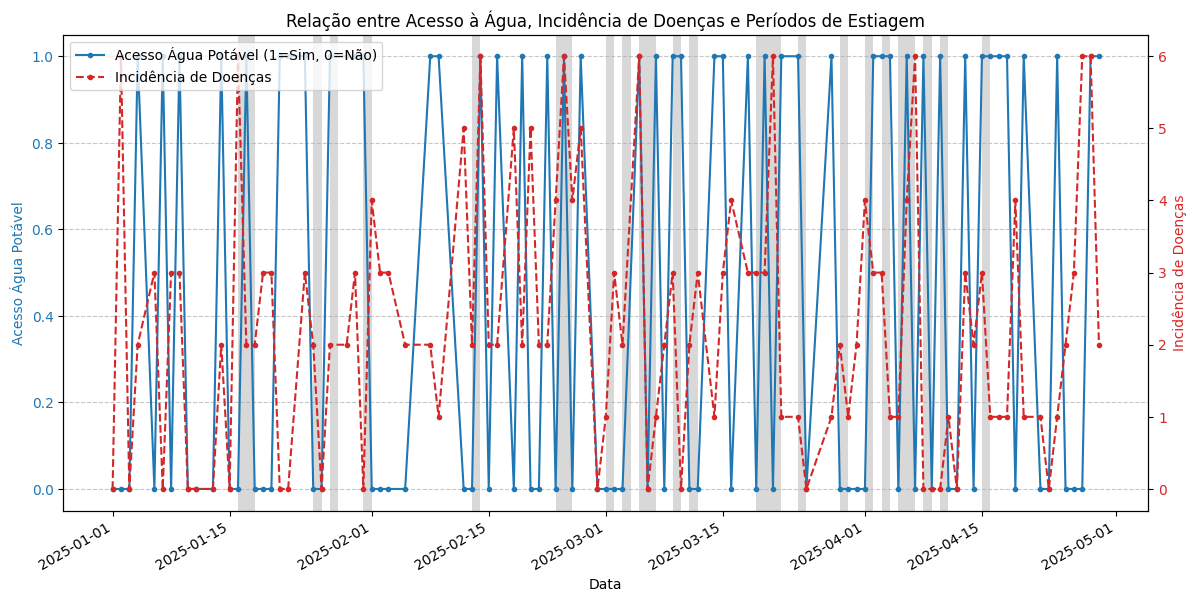
\includegraphics[width=1.4 \textwidth]{figures/grafico_pergunta_4.png}}
        \caption{Gráfico de Séries Temporais: Acesso à Água Potável e Incidência de Doenças}
        \label{fig:serie_temporal_acesso_agua_doencas}
    \end{figure}

    \textbf{Interpretação:} Períodos de Estiagem (barras cinzas): As barras cinzas marcam os períodos de seca.

    Acesso à Água Potável (linha azul): O acesso à água potável (valor 1 = Sim, 0 = Não) é intermitente. O acesso é cortado (cai para 0) precisamente durante os períodos de estiagem marcados pelas barras cinzas.

    Incidência de Doenças (linha vermelha tracejada): Assim como no Gráfico 2, a incidência de doenças tem picos agudos. Notavelmente, esses picos ocorrem exatamente durante ou logo após os períodos em que o acesso à água potável é interrompido.
    \vspace{0.5cm}

    \textbf{Resposta:} A análise sugere que existe uma relação direta entre a diminuição do acesso à água potável e o aumento da incidência de doenças, especialmente durante períodos de baixa precipitação. Durante os períodos de estiagem, o acesso à água potável diminui, o que está associado a um aumento na incidência de doenças.

    \section{Conclusão}
    A análise dos dados coletados e processados revelou insights significativos sobre os impactos das mudanças climáticas na agricultura local e na saúde da população. As respostas às perguntas centrais indicam que:
    \begin{enumerate}
        \item A região enfrenta uma forte estiagem que causa baixa umidade no solo, impactando diretamente e de forma negativa a produção agrícola.
        \item  As ondas de calor são um gatilho direto para o aumento de doenças na população, sugerindo a proliferação de doenças transmitidas por vetores (como dengue, que se beneficia do calor) ou problemas de saúde diretamente ligados à alta temperatura.
        \item A crise hídrica e agrícola se traduz diretamente em uma crise de segurança alimentar, tornando a população vulnerável à escassez de alimentos.
        \item A estiagem não só afeta a agricultura, mas também o abastecimento de água potável para a população. A falta de acesso à água segura está diretamente ligada a surtos de doenças, provavelmente de veiculação hídrica (cólera, diarreia, etc.) ou relacionadas à falta de higiene.
    \end{enumerate}

    Essas descobertas ressaltam a necessidade urgente de intervenções para mitigar os efeitos das mudanças climáticas na região, incluindo estratégias de gestão de água, práticas agrícolas sustentáveis e programas de saúde pública para lidar com o aumento das doenças. A colaboração entre as comunidades locais, autoridades governamentais e organizações não governamentais será crucial para enfrentar esses desafios e garantir a segurança hídrica e alimentar da população.

    \vspace{1cm}
    + Aluno: \author{Felipe Rafael Barbosa}

    + Telefone: (91) 9 9244-0421
\end{document}